%To compile as handout, use
%pdflatex "\def\ishandout{1} \input{filename.tex}"
%Defaults to non-handout mode (with slide reveals)
\ifdefined\ishandout
  \documentclass[handout]{beamer}
\else
  \documentclass{beamer}
\fi
 
\usepackage{econ103slides} 

\date{Lecture \# 8}
\begin{document} 

%%%%%%%%%%%%%%%%%%%%%%%%%%%%%%%%%%%%%%%%

\begin{frame}[plain]
	\titlepage 
	

\end{frame} 


%%%%%%%%%%%%%%%%%%%%%%%%%%%%%%%%%%%%%%%%
%Some macros for diagrams of random variables
\def\RVraw{(-2.5,0) circle [radius=1.7]
	(-2.5,0) circle [radius=1.7]
	(2.5,0) circle [radius=1.7]
	node [above left] at (-3.75,1.25) {$S$}
	node [above right] at (3.75,1.25) {$\mathbb{R}$}
	node [above] at (0,2) {$X\colon S \mapsto \mathbb{R}$}}
%%%%%%%%%%%%%%%%%%%%%%%%%%%%%%%%%%%%%%%%
%\begin{frame}
%  \frametitle{Random Variables}
%  \begin{quote}
%    A random variable is neither random nor a variable.
%  \end{quote}
%\begin{block}{Random Variable (RV): $X$}
%  A deterministic (i.e.\ non-random) function that assigns a numeric value to each basic outcome of a random experimnet.
%\end{block}
% 
%\begin{block}{Realization: $x$}
%A particular numeric value that an RV could take on. We write $\{X = x\}$ to refer to the \emph{event} that the RV $X$ took on the value $x$.  
%\end{block}
% 
%\begin{block}{Support Set (aka Support)}
%The set of all possible realizations of a RV.
%\end{block}
% 
%\end{frame}
%%%%%%%%%%%%%%%%%%%%%%%%%%%%%%%%%%%%%%%%%
%\begin{frame}
%  \frametitle{Random Variables (continued)}
%\begin{block}{Notation}
%Capital latin letters for RVs, e.g.\ $X,Y,Z$, and the corresponsing lowercase letters for their realizations, e.g.\ $x,y,z$.
%\end{block}
%
%\begin{block}{Intuition}
%  You can think of an RV as a machine that spits out random numbers: although the machine is deterministic, its inputs, the outcomes of a random experiment, are not.
%\end{block}
%\end{frame}
%%%%%%%%%%%%%%%%%%%%%%%%%%%%%%%%%%%%%%%%%%
%\begin{frame}
%\frametitle{Example: Coin Flip Random Variable}
%
%\begin{figure}
%\centering
%\begin{tikzpicture}
%\draw \RVraw;
%\draw [->] (-2.5,0.75) node [below]{Tails} to [out=35,in=145] (2.5,0.75) node [below]{$0$};
%\draw [->] (-2.5,-0.75) node [above]{Heads} to [out=315,in=225] (2.5,-0.75) node [above]{$1$};
%\end{tikzpicture}
%\caption{This random variable assigns numeric values to the random experiment of flipping a fair coin once: Heads is assigned 1 and Tails 0.}
%\end{figure}
%\end{frame}
%%%%%%%%%%%%%%%%%%%%%%%%%%%%%%%%%%%%%%%%%%%
%\begin{frame}
%  \frametitle{Which of these is a realization of the Coin Flip RV?\hfill
\includegraphics[scale = 0.05]{./images/clicker}}
%  \begin{enumerate}[(a)]
%    \item Tails
%    \item 2
%    \item 0 
%    \item Heads
%    \item 1/2
%  \end{enumerate}
%\end{frame}
%%%%%%%%%%%%%%%%%%%%%%%%%%%%%%%%%%%%%%%%%%%
%\begin{frame}
%  \frametitle{What is the support set of the Coin Flip RV?\hfill
\includegraphics[scale = 0.05]{./images/clicker}}
%  \begin{enumerate}[(a)]
%    \item $\left\{ \mbox{Heads}, \mbox{Tails} \right\}$ 
%    \item 1/2 
%    \item 0 
%    \item $\left\{ 0,1 \right\}$
%    \item 1
%  \end{enumerate}
%\end{frame}
%%%%%%%%%%%%%%%%%%%%%%%%%%%%%%%%%%%%%%%%%%%
%\begin{frame}
%  \frametitle{Let $X$ denote the Coin Flip RV \hfill
\includegraphics[scale = 0.05]{./images/clicker}}
%  What is $P\left( X=1 \right)$?
%
%  \vspace{1em}
%
%  \begin{enumerate}[(a)]
%    \item 0 
%    \item 1  
%    \item 1/2 
%    \item Not enough information to determine
%  \end{enumerate}
%\end{frame}
%%%%%%%%%%%%%%%%%%%%%%%%%%%%%%%%%%%%%%%%%%%
%\begin{frame}
%  \frametitle{Two Kinds of RVs: Discrete and Continuous}
%  \begin{description}
%    \item[Discrete] support set is finite or countable , e.g.\ $\left\{ 0,1 \right\}$,  $\left\{ \hdots, -2, -1, 0, 1, 2,\hdots \right\}$
%    \item[Continuous] support set is \emph{uncountable} e.g.\ $[-1,1]$, $\mathbb{R}$.
%  \end{description}
%
%  \vspace{1em}
%
%  \alert{Start with the discrete case since it's easier, but most of the ideas we learn will carry over to the continuous case.}
%\end{frame}
%%%%%%%%%%%%%%%%%%%%%%%%%%%%%%%%%%%%%%%%%%%
%\begin{frame}
%
%\centering \Huge Discrete Random Variables I
%
%\end{frame}
%%%%%%%%%%%%%%%%%%%%%%%%%%%%%%%%%%%%%%%%%
%\begin{frame}
%\frametitle{Probability Mass Function (pmf)}
% A function that gives $P(X=x)$ for any realization $x$ in the support set of a discrete RV $X$. We use the following notation for the pmf:
% $$p(x) = P(X =x)$$
%
% 
%
%\begin{alertblock}{Plug in a realization $x$, get out a probability  $p(x)$.}\end{alertblock}
%
% 
%
%
%\end{frame}
%%%%%%%%%%%%%%%%%%%%%%%%%%%%%%%%%%%%%%%%%
%\begin{frame}
%\frametitle{Probability Mass Function for Coin Flip RV}
%
%\begin{columns}
%\column{0.25\textwidth}
%$$X = \left\{ \begin{array}{l}  0, \mbox{Tails}\\ 1, \mbox{Heads}\end{array} \right.$$
%
%\begin{eqnarray*}
%	p(0) &=& 1/2\\
%	p(1) &=& 1/2
%\end{eqnarray*}
%
%
%\column{0.75\textwidth}
%\begin{figure}
%\centering
%\begin{tikzpicture}[scale = 1.5]
%\draw [<->] (0,2) node [above]{$p(x)$} -- (0,0) -- (3,0) node [right]{$x$};
%\draw [blue, thick] (0.75,0) node [black, below]{0} -- (0.75,1.5);
%\draw [blue, thick] (2.25,0) node [black, below]{1} -- (2.25,1.5);
%\draw [dashed, gray] (0, 1.5) node [black, left]{$1/2$} -- (3,1.5);
%\draw [fill=blue] (2.25,1.51) circle [radius = 0.05];
%\draw [fill=blue] (0.75,1.51) circle [radius = 0.05];
%\end{tikzpicture}
%\caption{Plot of pmf for Coin Flip Random Variable}
%\end{figure}
%\end{columns}
%
%
%\end{frame}
%%%%%%%%%%%%%%%%%%%%%%%%%%%%%%%%%%%%%%%%%
%
%
%\begin{frame}
%\frametitle{Important Note about Support Sets}
%Whenever you write down the pmf of a RV, it is \alert{crucial} to also write down its Support Set. Recall that this is the set of \alert{\emph{all possible realizations for a RV}}. Outside of the support set, all probabilities are zero. In other words, the pmf is \alert{only defined} on the support.
%
%\end{frame}
%%%%%%%%%%%%%%%%%%%%%%%%%%%%%%%%%%%%%%%%
\begin{frame}
\frametitle{Recall: Properties of Probability Mass Functions}

If $p(x)$ is the pmf of a random variable $X$, then
\begin{enumerate}[(i)]
	\item $0\leq p(x) \leq 1$ for all $x$ \vspace{1em}
	\item $\displaystyle \sum_{\mbox{all } x} p(x) = 1$
\end{enumerate}

\vspace{0.75em}
where ``all $x$'' is shorthand for ``all $x$ in the support of $X$.''
%%%%%%%%%%%%%%%%%%%%%%%%%%%%%%%%%%%%%%%%

\end{frame}
%%%%%%%%%%%%%%%%%%%%%%%%%%%%%%%%%%%%%%%%

\begin{frame}
\frametitle{Cumulative Distribution Function (CDF)}
\framesubtitle{This Def.\ is \alert{the same} for continuous RVs.}

The CDF gives the probability that a RV $X$ \alert{does not exceed} a specified threshold $x_0$, as a function of $x_0$
	$$F(x_0) = P(X \leq x_0)$$

\begin{alertblock}{Important!}
The threshold $x_0$ is allowed to be \emph{any real number}. In particular, it doesn't have to be in the support of $X$! 
\end{alertblock}

\end{frame}
%%%%%%%%%%%%%%%%%%%%%%%%%%%%%%%%%%%%%%%%
\begin{frame}
\frametitle{Discrete RVs: Sum the pmf to get the CDF}
\begin{center}
	\alert{$$\boxed{F(x_0) = \sum_{x\leq x_0} p(x)}$$}
\end{center}

\small
 
\begin{block}{Why?}
The events $\{X = x\}$ are mutually exclusive, so we sum to get the probability of their union for all $x\leq x_0$:
	$$F(x_0) = P(X \leq x_0)=   P\left(\bigcup_{x\leq x_0}\{X = x\}\right) =   \sum_{x \leq x_0} P(X = x) =   \sum_{x \leq x_0} p(x)$$
\end{block}

\end{frame}


%%%%%%%%%%%%%%%%%%%%%%%%%%%%%%%%%%%%%%%%

\begin{frame}[t]
	% \frametitle{Sum the pmf to get the CDF}
	% \framesubtitle{Coin-Flip Random Variable}

\begin{columns}[t]
	\column{0.48\textwidth}
	\begin{block}{Probability Mass Function}
	\begin{figure}
\centering
\begin{tikzpicture}[scale = 1.2]
\draw [<->] (0,2) node [above]{$p(x)$} -- (0,0) -- (3,0) node [right]{$x$};
\draw [blue, thick] (0.75,0) node [black, below]{0} -- (0.75,1.5);
\draw [blue, thick] (2.25,0) node [black, below]{1} -- (2.25,1.5);
\draw [dashed, gray] (0, 1.5) node [black, left]{$1/2$} -- (3,1.5);
\draw [fill=blue] (2.25,1.51) circle [radius = 0.05];
\draw [fill=blue] (0.75,1.51) circle [radius = 0.05];
\end{tikzpicture}
\end{figure}
\begin{eqnarray*}
	p(0) &=& 1/2\\
	p(1) &=& 1/2
\end{eqnarray*}
	\end{block}

	\column{0.48\textwidth}
	\begin{block}{Cumulative Dist.\ Function}
\begin{figure}
\centering
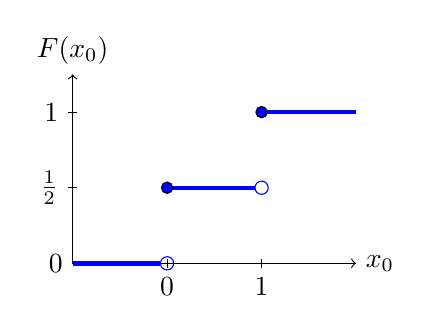
\begin{tikzpicture}[scale = 1.2]
\draw [<->] (0,2) node [above]{$F(x_0)$} -- (0,0) -- (3,0) node [right]{$x_0$};
\draw (-0.05, 1.6) node [black, left]{$1$} -- (0.05,1.6);
\draw (-0.05, 0.8) node [black, left]{$\frac{1}{2}$} -- (0.05,0.8);
\draw [blue, ultra thick] (0,0) -- (0.93,0);
\draw [blue, ultra thick] (1,0.8) -- (1.93,0.8);
\draw [blue, ultra thick] (2,1.6) -- (3,1.6);
\draw (1,-0.05) node [black, below]{0} -- (1,0.05);
\draw (2,-0.05) node [black, below]{1} -- (2,0.05);
\draw (0,0) node [black, left]{$0$};
\draw [blue] (1,0) circle [radius = 0.07];
\draw [fill = blue] (1,0.8) circle [radius = 0.06];
\draw [blue] (2,0.8) circle [radius = 0.07];
\draw [fill = blue] (2,1.6) circle [radius = 0.06];
\end{tikzpicture}
\end{figure}
\begin{eqnarray*}
	F(x_0) = \left\{\begin{array}{ll} 0,& x_0 < 0\\ \frac{1}{2}, &0\leq x_0 < 1\\ 1,& x_0 \geq 1\end{array}\right.
\end{eqnarray*}
	\end{block}
\end{columns}
\end{frame}

%%%%%%%%%%%%%%%%%%%%%%%%%%%%%%%%%%%%%%%%

\begin{frame}
\frametitle{Properties of CDFs}
\framesubtitle{These are also true for continuous RVs.}
	\begin{enumerate}
		\item $\lim_{x_0 \rightarrow \infty} F(x_0) = 1$
		\item $\lim_{x_0 \rightarrow -\infty} F(x_0) = 0$
		\item Non-decreasing: $x_0 < x_1 \Rightarrow F(x_0)\leq F(x_1)$
		\item Right-continuous (``open'' versus ``closed'' on prev.\ slide)
	\end{enumerate}
	
	
	 
	
	
\vspace{1em}
\begin{alertblock}{Since $F(x_0) = P(X\leq x_0)$,  we have $0\leq F(x_0)\leq 1$ for all $x_0$}\end{alertblock}
\end{frame}
%%%%%%%%%%%%%%%%%%%%%%%%%%%%%%%%%%%%%%%%

\begin{frame}
\frametitle{Bernoulli Random Variable -- Generalization of Coin Flip}
\small
\begin{block}{Support Set}
$\{0,1\}$ -- 1 traditionally called ``success,'' 0 ``failure''
\end{block}

\begin{block}{Probability Mass Function}
	\begin{eqnarray*}
		p(0) &=& 1-p\\
		p(1) &=& p
	\end{eqnarray*}

	\begin{block}{Cumulative Distribution Function}
\begin{eqnarray*}
	F(x_0) = \left\{\begin{array}{ll} 0,& x_0 < 0\\ 1-p, &0\leq x_0 < 1\\ 1,& x_0 \geq 1\end{array}\right.
\end{eqnarray*}
\end{block}
\end{block}

\end{frame}
%%%%%%%%%%%%%%%%%%%%%%%%%%%%%%%%%%%%%%%%
\begin{frame}
	\frametitle{\href{http://fditraglia.shinyapps.io/binom_cdf/}{http://fditraglia.shinyapps.io/binom\_cdf/}}
\framesubtitle{Set the second slider to 1 and play around with the others.}

\begin{figure}
	\fbox{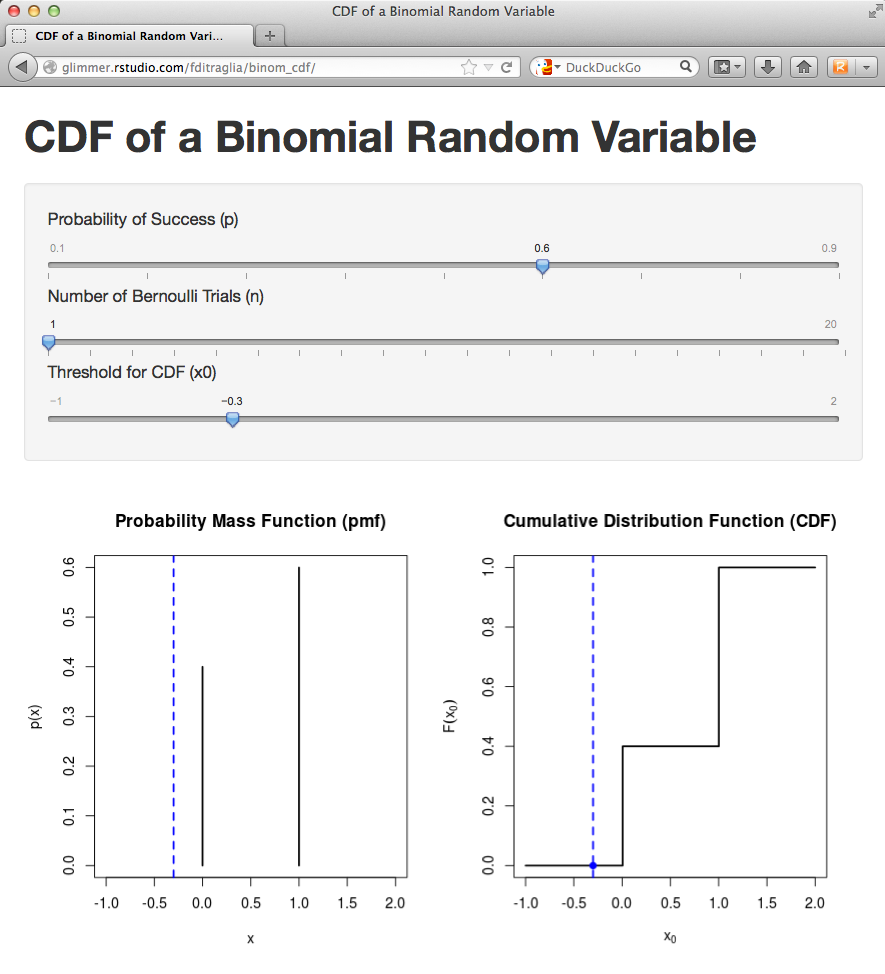
\includegraphics[scale = 0.2]{./images/binom_cdf_screenshot}}
\end{figure}

\end{frame}


%%%%%%%%%%%%%%%%%%%%%%%%%%%%%%%%%%%%%%%%

\begin{frame}
\frametitle{Average Winnings Per Trial \hfill 
\includegraphics[scale = 0.05]{./images/clicker}}
If the realizations of the coin-flip RV were \alert{payoffs}, how much would you expect to win per play \emph{on average} in a long sequence of plays?
$$X = \left\{ \begin{array}{l}  \$0, \mbox{Tails}\\ \$1, \mbox{Heads}\end{array} \right.$$
\end{frame}
%%%%%%%%%%%%%%%%%%%%%%%%%%%%%%%%%%%%%%%%
\begin{frame}
\frametitle{Expected Value (aka Expectation)}
The expected value of a discrete RV $X$ is given by
	$$E[X] = \sum_{\mbox{all} \; x} x \cdot p(x)$$

  \vspace{1em}
  \alert{In other words, the expected value of a discrete RV is the \emph{probability-weighted average of its realizations}.}

  \vspace{1em}

  \begin{block}{Notation}
    We sometimes write $\mu$ as shorthand for $E[X]$.  \end{block}
\end{frame}
%%%%%%%%%%%%%%%%%%%%%%%%%%%%%%%%%%%%%%%%
\begin{frame}
  \frametitle{Expected Value of Bernoulli RV}
$$X = \left\{ \begin{array}{l}  0, \mbox{Failure: } 1-p\\ 1, \mbox{Success: } p\end{array} \right.$$

\vspace{2em}
 
$$\sum_{\mbox{all} \; x} x \cdot p(x) = 0 \cdot (1-p) + 1 \cdot p = p$$
\end{frame}
%%%%%%%%%%%%%%%%%%%%%%%%%%%%%%%%%%%%%%%%
\begin{frame}
  \frametitle{Your Turn to Caculate an Expected Value \hfill
\includegraphics[scale = 0.05]{./images/clicker}}
  Let $X$ be a random variable with support set $\left\{ 1,2,3 \right\}$ where $p(1)=p(2)=1/3$. Calculate $E[X]$.

  \pause

  \vspace{1em}
  \begin{equation*}
    E[X] = \sum_{\mbox{all }x} x \cdot p(x) = 1 \times 1/3 + 2 \times 1/3 + 3 \times 1/3 = 2
  \end{equation*}
\end{frame}
%%%%%%%%%%%%%%%%%%%%%%%%%%%%%%%%%%%%%%%%

\begin{frame}
\frametitle{Random Variables and Parameters}



\begin{block}{Notation: $X \sim$ Bernoulli$(p)$}
Means $X$ is a Bernoulli RV with $P(X = 1) = p$ and $P(X= 0) = 1-p$. The tilde is read ``distributes as.''

\end{block}


\begin{block}{Parameter}
Any constant that appears in the definition of a RV, here $p$. 
\end{block}


\end{frame}
%%%%%%%%%%%%%%%%%%%%%%%%%%%%%%%%%%%%%%%%

\begin{frame}
\frametitle{Constants Versus Random Variables}

 \alert{This is a crucial distinction that students sometimes miss:}
 \vspace{1em}
 

 		\begin{block}{Random Variables}
 			\begin{itemize}
 			\item Suppose $X$ is a RV -- the values it takes on are random
 			\item A function $g(X)$ of a RV is itself a RV as we'll learn today.
 			\end{itemize}
 		\end{block}
 
 		\begin{block}{Constants}
 			\begin{itemize}
 				\item $E[X]$ is a constant (you should convince yourself of this)
 				\item Realizations $x$ are constants. What is random is \emph{which} realization the RV takes on.
 				\item Parameters are constants (e.g.\ $p$ for Bernoulli RV)
 				\item Sample size $n$ is a constant
 			\end{itemize}
 		\end{block} 

\end{frame}
%%%%%%%%%%%%%%%%%%%%%%%%%%%%%%%%%%%%%%%%
\begin{frame}
\Huge \centering The St.\ Petersburg Game

\end{frame}
%%%%%%%%%%%%%%%%%%%%%%%%%%%%%%%%%%%%%%%%
\begin{frame}
\frametitle{How Much Would You Pay?\hfill 
\includegraphics[scale = 0.05]{./images/clicker}}
How much would you be willing to pay for the right to play the following game?

\vspace{1em}
\begin{quote}
Imagine a fair coin. The coin is tossed once. If it falls heads, you receive a prize of \$2 and the game stops. If not, it is tossed again. If it falls heads on the second toss, you get \$4 and the game stops. If not, it is tossed again. If it falls heads on the third toss, you get \$8 and the game stops, and so on. The game stops after the first head is thrown. If the first head is thrown on the $x^{th}$ toss, the prize is \$$2^x$
\end{quote}

\end{frame}
%%%%%%%%%%%%%%%%%%%%%%%%%%%%%%%%%%%%%%%%
\begin{frame}
\frametitle{$X =$ Trial Number of First Head}
\begin{table}
\begin{tabular}{c|c|c|c}
	$x$ & $2^x$ & $p(x)$& $2^x \cdot p(x)$\\
		\hline \uncover<2->{
	1&2&1/2&1\\
	2&4&1/4&1\\
	3&8&1/8&1\\}\uncover<3->{
	$\vdots$&$\vdots$&$\vdots$&$\vdots$\\
	n&$2^n$&$1/2^n$&1\\
	$\vdots$&$\vdots$&$\vdots$&$\vdots$}
\end{tabular}
\end{table}
$$E[Y] = \sum_{\mbox{all } x} 2^x\cdot p(x) = \uncover<4->{1 + 1 + 1 + \hdots}\uncover<5->{ = \infty}$$
\end{frame}
%%%%%%%%%%%%%%%%%%%%%%%%%%%%%%%%%%%%%%%%

\begin{frame}
\begin{center}
\Huge Functions of Random Variables are Themselves Random Variables
\end{center}

\end{frame}
%%%%%%%%%%%%%%%%%%%%%%%%%%%%%%%%%%%%%%%%

\begin{frame}
\frametitle{Example: Function of Bernoulli RV}
\fbox{Let $Y=e^X$ where $X \sim \mbox{Bernoulli}(p)$}
\vspace{2em}

\begin{block}{Support of $Y$} \pause
$\{e^0, e^1\} =\{1, e\}$
\end{block}

\begin{block}{Probability Mass Function for $Y$} \pause
	$$p_Y(y) = \left\{\begin{array}{ll}p& y =e\\ 1-p& y = 1\\ 0& \mbox{otherwise}\end{array}\right.$$
\end{block}

\end{frame}
%%%%%%%%%%%%%%%%%%%%%%%%%%%%%%%%%%%%%%%%
\begin{frame}
\frametitle{Expectation: Function of Bernoulli RV}
\fbox{Let $Y=e^X$ where $X \sim \mbox{Bernoulli}(p)$}
\vspace{2em}

\begin{block}{Probability Mass Function for $Y$} 
	$$p_Y(y) = \left\{\begin{array}{ll}p& y =e\\ 1-p& y = 1\\ 0& \mbox{otherwise}\end{array}\right.$$
\end{block}

\begin{block}{Expectation of $Y = e^X$}\pause
$$\sum_{y \in \{1, e\}} y \cdot p_Y(y) =\pause (1-p) \cdot 1 + p \cdot e = 1 + p(e - 1)$$
\end{block}




\end{frame}
%%%%%%%%%%%%%%%%%%%%%%%%%%%%%%%%%%%%%%%%
\begin{frame}
\frametitle{Expectation: Function of Bernoulli RV}
\fbox{Let $Y=e^X$ where $X \sim \mbox{Bernoulli}(p)$}
\vspace{2em}



\begin{block}{Expectation of the Function}
$$\sum_{y \in \{1, e\}} y \cdot p_Y(y) = (1-p) \cdot 1 + p \cdot e = 1 + p(e - 1)$$
\end{block}

\begin{block}{Function of the Expectation}
$$e^{E[X]} = e^p $$
\end{block}



\end{frame}
%%%%%%%%%%%%%%%%%%%%%%%%%%%%%%%%%%%%%%%%


\begin{frame}
\huge $$E[g(X)] \neq g(E[X])$$
\begin{center}
	\large (Expected value of Function $\neq$ Function of Expected Value)
\end{center}


\end{frame}
%%%%%%%%%%%%%%%%%%%%%%%%%%%%%%%%%%%%%%%%

\begin{frame}
\frametitle{Expectation of a Function of a Discrete RV}
Let $X$ be a random variable and $g$ be a function. Then:
$$\boxed{E[g(X)] = \sum_{\mbox{all } x} g(x) p(x)}$$


 \alert{This is how we proceeded in the St.\ Petersburg Game Example}
\end{frame}
%%%%%%%%%%%%%%%%%%%%%%%%%%%%%%%%%%%%%%%%
\begin{frame}
\frametitle{Your Turn: Calculate $E[X^2]$ \hfill 
\includegraphics[scale = 0.05]{./images/clicker}}
$X$ has support $\{-1, 0, 1\}$, $p(-1) = p(0) = p(1) = 1/3$.
\pause

\begin{eqnarray*}
 E[X^2] &=&  \sum_{\mbox{all } x} x^2 p(x) = \sum_{x \in \{-1, 0, 1\}} x^2 p(x) \\ \\ \pause
 	&=& (-1)^2 \cdot (1/3) + (0)^2 \cdot (1/3) + (1)^2 \cdot (1/3)\\ \pause
 	&=& 1/3 + 1/3\\ 
 	&=& 2/3 \approx 0.67
\end{eqnarray*}

\end{frame}
%%%%%%%%%%%%%%%%%%%%%%%%%%%%%%%%%%%%%%%
%\begin{frame}
  %\frametitle{Why Random Variables?}
  %Use as a model for population. No longer talk about population size $N$, because this turns out to be irrelevant. Explain why with a simple example. This slide should probably come after I actually introduce Bernoulli RV, etc. Treat population relative frequencies as probabilities rather than counts divided by $N$. Defined probability as long-run relative frequency and here we would think of repeatedly sampling from the population. Also we never know $N$ in practice. Emphasize that from the perspective of sampling, $N$ is irrelevant. Give a simple urn example. Try to distinguish continuous and discrete. Then again, maybe it's still too early for them to digest this.
  %Many random experiments are ``the same'' from a probabilistic perspective. Focus on only the essential details. Examples.
%\end{frame}
%%%%%%%%%%%%%%%%%%%%%%%%%%%%%%%%%%%%%%%

%%%%%%%%%%%%%%%%%%%%%%%%%%%%%%%%%%%%%%%%

\begin{frame}
\frametitle{Linearity of Expectation}
\framesubtitle{Holds for Continuous RVs as well, but proof is different.}
Let $X$ be a RV and $a,b$ be constants. Then:
	$$E[a + bX] = a + bE[X]$$
\vspace{2em}
\begin{alertblock}{This is one of the most important facts in the course: the special case in which $E[g(X)] = g(E[X])$ is $g = a+bX$.}
\end{alertblock}
\end{frame}
%%%%%%%%%%%%%%%%%%%%%%%%%%%%%%%%%%%%%%%%
\begin{frame}
\frametitle{Example: Linearity of Expectation \hfill 
\includegraphics[scale = 0.05]{./images/clicker} }
Let $X \sim \mbox{Bernoulli}(1/3)$ and define $Y = 3X + 2$
\vspace{1em}

\begin{enumerate}
  \item What is $E[X]$? \pause \hspace{2em} \alert{$E[X] = 0 \times 2/3 + 1 \times 1/3 = 1/3$} \pause
  \item What is $E[Y]$? \pause \hspace{2em} \alert{$E[Y] = E[3X + 2] = 3E[X] + 2 = 3$}
\end{enumerate}
\end{frame}
%%%%%%%%%%%%%%%%%%%%%%%%%%%%%%%%%%%%%%%%

\begin{frame}
\frametitle{Proof: Linearity of Expectation For Discrete RV}

\begin{eqnarray*}
	E[a + bX] &=& \sum_{\mbox{all } x}  (a + bx) p(x)\\ \\
	 &=&  \sum_{\mbox{all } x} p(x) \cdot a + \sum_{\mbox{all } x}p(x) \cdot bx\\ \\
	&=&  a\sum_{\mbox{all } x} p(x) + b\sum_{\mbox{all } x} x \cdot p(x) \\ \\
	&=&  a + b E[X]
\end{eqnarray*}


\end{frame}
%%%%%%%%%%%%%%%%%%%%%%%%%%%%%%%%%%%%%%%%

%\begin{frame}
%\frametitle{Variance and Standard Deviation of a RV}
%\framesubtitle{The Defs are the same for continuous RVs, but the method of calculating will differ.}
%
%\begin{block}{Variance (Var)}
%	$$\sigma^2 = Var(X) = E\left[ (X - \mu)^2\right] = E\left[ (X - E[X])^2\right]$$
%\end{block}
%
%
%\begin{block}{Standard Deviation (SD)}
%$$\sigma = \sqrt{\sigma^2} = SD(X)$$
%\end{block}
%
%
%\end{frame}
%%%%%%%%%%%%%%%%%%%%%%%%%%%%%%%%%%%%%%%%%
%\begin{frame}
%\frametitle{Key Point}
%
%\alert{Variance and std.\ dev.\ are \emph{expectations of functions of a RV}} 
%
%\vspace{1em}
%
%It follows that: 
%\begin{enumerate}
%\item Variance and SD are constants
%\item To derive facts about them you can use the facts you know about expected value
%\end{enumerate}
%\end{frame}
%%%%%%%%%%%%%%%%%%%%%%%%%%%%%%%%%%%%%%%%%
%\begin{frame}
%\frametitle{How To Calculate Variance for Discrete RV?}
%\framesubtitle{Remember: it's just a function of $X$!}
%
%
%Recall that	$\displaystyle \mu = E[X] = \sum_{\mbox{all } x} xp(x)$
%
%
%\vspace{3em}
%
%$$Var(X) = E\left[ (X - \mu)^2 \right] =\sum_{\mbox{all } x} (x - \mu)^2 p(x)$$
%
%
%\end{frame}
%%%%%%%%%%%%%%%%%%%%%%%%%%%%%%%%%%%%%%%%%
%\begin{frame}
%\frametitle{Shortcut Formula For Variance}
%
%This is \emph{not} the definition, it's a shortcut for doing calculations:
%\begin{eqnarray*}
%	Var(X) = E\left[ (X - \mu)^2 \right] = E[X^2] - \left(E[X]\right)^2
%\end{eqnarray*}
%
%\alert{We'll prove this in an upcoming lecture.}
%
%\end{frame}
%
%%%%%%%%%%%%%%%%%%%%%%%%%%%%%%%%%%%%%%%%%
%\begin{frame}
%\frametitle{Example: The Shortcut Formula \hfill 
\includegraphics[scale = 0.05]{./images/clicker}}
%Let $X\sim \mbox{Bernoulli}(1/2)$.
%\begin{enumerate}
%  \item What is $E[X]$? \hspace{1em} \pause \alert{$E[X] = 0 \times 1/2 + 1 \times 1/2 = 1/2$} \pause
%    \item What is $E[X^2]$? \pause \hspace{1em} \alert{$E[X^2] = 0^2 \times 1/2 + 1^2 \times 1/2 = 1/2$} \pause
%    \item What is $Var(X)$? \pause \hspace{1em} \alert{$E[X^2] - \left( E[X] \right)^2 = 1/2 - (1/2)^2 = 1/4$} 
%\end{enumerate}
%\end{frame}
%%%%%%%%%%%%%%%%%%%%%%%%%%%%%%%%%%%%%%%%%
%
%
%\begin{frame}
%\frametitle{Variance of Bernoulli RV -- via the Shortcut Formula}
%
%\begin{block}{Step 1 -- $E[X]$} 
%$\mu = E[X] = \displaystyle \sum_{x \in \{0,1\}} p(x) \cdot x = (1-p) \cdot 0 + p \cdot 1 = p$
%\end{block}
%
%
%\begin{block}{Step 2 -- $E[X^2]$} 
%\begin{eqnarray*}
%	E[X^2] = \sum_{x \in \{0,1\}} x^2 p(x) = 0^2 (1-p) + 1^2 p = p
%\end{eqnarray*}
%\end{block}
%
%
%\begin{block}{Step 3 -- Combine with Shortcut Formula} 
%\begin{eqnarray*}
%	\sigma^2 = Var[X] = E[X^2] - \left(E[X]\right)^2 = \ p - p^2 =  p(1-p)
%\end{eqnarray*}
%\end{block}
%
%
%\end{frame}
%%%%%%%%%%%%%%%%%%%%%%%%%%%%%%%%%%%%%%%%%
%
%
%
%\begin{frame}
%\frametitle{Variance of Bernoulli RV -- Without Shortcut}
%
%\alert{You will fill in the missing steps on Problem Set 5.}
%
%\begin{eqnarray*}
%	\sigma^2 &=& Var(X) = \sum_{x \in \{0,1\}} (x - \mu)^2 p(x)\\
%	 &=& \sum_{x \in \{0,1\}} (x - p)^2 p(x)\\
%	 &\vdots &\\ 
%	 &=&p(1-p)
%\end{eqnarray*}
%
%%%%%%%%%%%%%%%%%%%%%%%%%%%%%%%%%%%%%%%%%
%
%
%\end{frame}
%
%\begin{frame}
%\frametitle{Variance of a Linear Function  \hfill 
\includegraphics[scale = 0.05]{./images/clicker} }
%Suppose $X$ is a random variable with $Var(X) = \sigma^2$ and $a,b$ are constants. What is $Var(a + bX)$? 
%\begin{enumerate}[(a)]
%	\item $\sigma^2$
%	\item $a + \sigma^2$
%	\item $b \sigma^2$
%	\item $a + b \sigma^2$
%	\item $b^2 \sigma^2$
%\end{enumerate}
%
%\end{frame}
%%%%%%%%%%%%%%%%%%%%%%%%%%%%%%%%%%%%%%%%%
%\begin{frame}
%	\frametitle{Variance and SD are \emph{NOT} Linear}
%
%\begin{eqnarray*}
%Var(a + bX) &= &b^2 \sigma^2 \\\\
%	SD(a + bX)&=& |b| \sigma
%\end{eqnarray*}
%
%\vspace{2em}
%\begin{block}{These should look familiar from the related results for sample variance and std.\ dev. that you worked out on an earlier problem set.}
%
%\end{block}
%
%\end{frame}
%%%%%%%%%%%%%%%%%%%%%%%%%%%%%%%%%%%%%%%%%
%\begin{frame}
%\frametitle{Variance of a Linear Transformation}
%
%\begin{eqnarray*}
% Var(a + bX) &=& E\left[\left\{(a+bX) - E(a+bX)\right\}^2 \right] \\ 
% 	&=& E\left[\left\{(a+bX) - (a+bE[X])\right\}^2 \right] \\
% 	&=&E\left[\left(bX - bE[X]\right)^2 \right] \\ 
% 	&=&E[b^2 (X - E[X])^2]\\ 
% 	&=& b^2 E[(X-E[X])^2]\\ 
% 	&=& b^2 Var(X) = b^2 \sigma^2
%\end{eqnarray*}
%\alert{The key point here is that variance is defined in terms of expectation and expectation is linear.}
%
%\end{frame}
%%%%%%%%%%%%%%%%%%%%%%%%%%%%%%%%%%%%%%%%%
%\begin{frame}
%	\begin{center}
%		\Huge Binomial Random Variable	\\
%		\large What we get if we sum a bunch of indep.\ Bernoulli RVs
%	\end{center}
%\end{frame}
%
%%%%%%%%%%%%%%%%%%%%%%%%%%%%%%%%%%%%%%%%%
%
%\begin{frame}
%\frametitle{Binomial Random Variable}
%Let $X = $ the sum of $n$ independent Bernoulli trials, each with probability of success $p$.  \alert{Then we say that:
%		$X \sim \mbox{Binomial}(n,p)$} 
%
%\vspace{2em}
%\begin{block}{Parameters}
%$p =$ probability of ``success,'' $n=$ \# of trials
%\end{block}
%\begin{block}{Support} 
%$\{0, 1, 2, \hdots, n\}$ 
%\end{block}
%\begin{block}{Probability Mass Function (pmf)} 
%$$p(x) = {n \choose x} p^x (1-p)^{n-x}$$ 
%\end{block}
%\end{frame}
%%%%%%%%%%%%%%%%%%%%%%%%%%%%%%%%%%%%%%%%%
%
%\begin{frame}
%	\frametitle{\href{https://fditraglia.shinyapps.io/binom_cdf/}{http://fditraglia.shinyapps.io/binom\_cdf/}}
%\framesubtitle{Try playing around with all three sliders. If you set the second to 1 you get a Bernoulli.}
%
%\begin{figure}
%	\fbox{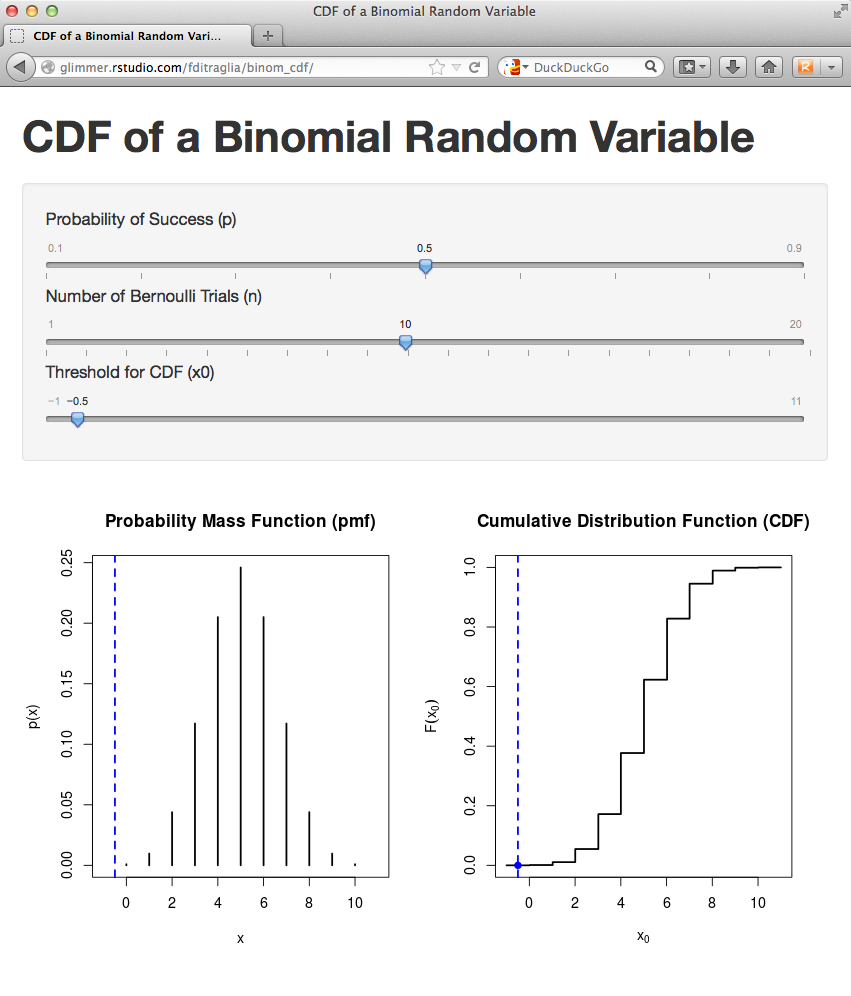
\includegraphics[scale = 0.2]{./images/binom_cdf_screenshot2}}
%\end{figure}
%
%\end{frame}
%
%%%%%%%%%%%%%%%%%%%%%%%%%%%%%%%%%%%%%%%%%
%
%
%\begin{frame}
%	\frametitle{\href{http://fditraglia.github.com/Econ103Public/Rtutorials/Bernoulli_Binomial.html}{\small http://fditraglia.github.com/Econ103Public/Rtutorials/Bernoulli\_Binomial.html}}
%
%\framesubtitle{Source Code on my \href{https://github.com/fditraglia/Econ103Public/blob/master/Rtutorials/Bernoulli_Binomial.R}{\fbox{Github Page}}}
%
%
%
%\begin{figure}
%	\fbox{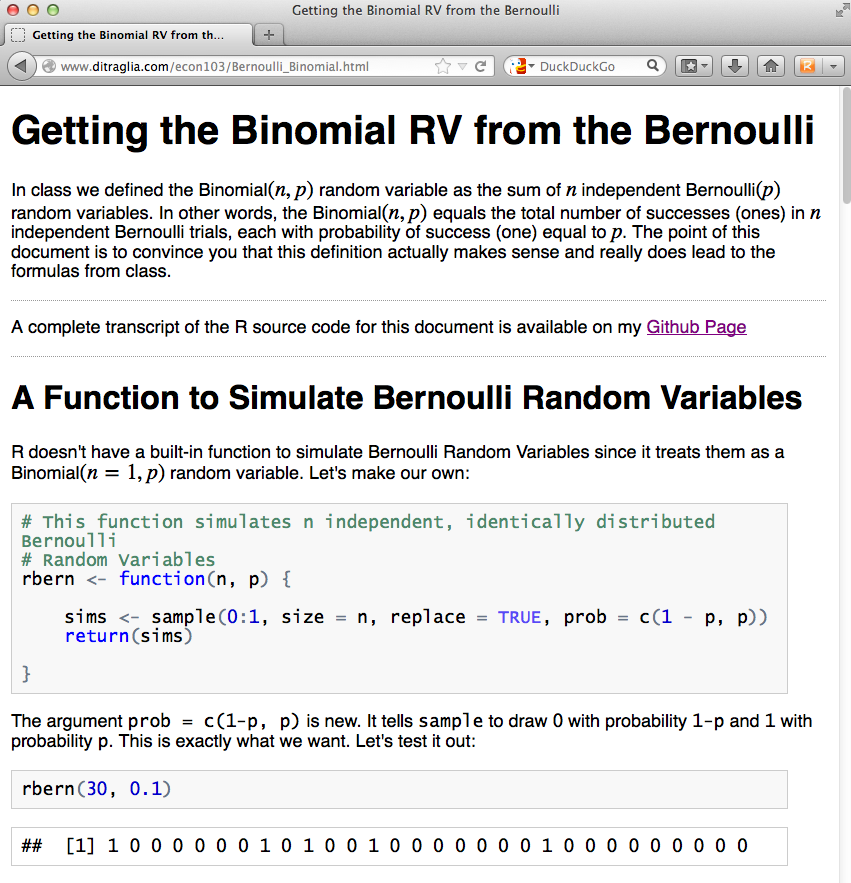
\includegraphics[scale = 0.15]{./images/binom_bernoulli_sim_screenshot}}
%\end{figure}
%
%\begin{alertblock}{Don't forget this!}
% Binomial RV counts up the \emph{total} number of successes (ones) in $n$ indep.\ Bernoulli trials, each with prob.\ of success $p$.
%\end{alertblock}
%
%\end{frame}
%
%%%%%%%%%%%%%%%%%%%%%%%%%%%%%%%%%%%%%%%%%
%
%\begin{frame}
%\frametitle{Where does the Binomial pmf come from? 
\includegraphics[scale = 0.05]{./images/clicker} }
%\begin{block}{Question}
%Suppose we flip a fair coin 3 times. What is the probability that we get exactly 2 heads?
%\end{block}
%
%\pause
%
%\begin{block}{Answer}
%Three basic outcomes make up this event: $\{HHT, HTH, THH\}$, each has probability $1/8 = 1/2 \times 1/2 \times 1/2$. Basic outcomes are mutually exclusive, so sum to get \alert{$3/8 = 0.375$}
%\end{block}
%
%\end{frame}
%%%%%%%%%%%%%%%%%%%%%%%%%%%%%%%%%%%%%%%%%
%\begin{frame}
%\frametitle{Where does the Binomial pmf come from?}
%\begin{block}{Question}
%Suppose we flip an \emph{unfair} coin 3 times, where the probability of heads is 1/3. What is the probability that we get exactly 2 heads?
%\end{block}
%
%
%
%\begin{block}{Answer}
%  No longer true that \emph{all} basic outcomes are equally likely, but those with exactly two heads \emph{\alert{still are}} 
%	\begin{eqnarray*}
%	 P(HHT) &=&  (1/3)^2 (1 - 1/3) =  2/27\\ 
%	 P(THH) &=&2/27\\ 
%	 P(HTH) &=&2/27 
%	\end{eqnarray*}
%	Summing gives \alert{$2/9 \approx 0.22$}
%\end{block}
%\end{frame}
%%%%%%%%%%%%%%%%%%%%%%%%%%%%%%%%%%%%%%%%%
%\begin{frame}
%  \frametitle{Where does the Binomial pmf come from?}
%\framesubtitle{Starting to see a pattern?}
%
%Suppose we flip an unfair coin \emph{4} times, where the probability of heads is 1/3. What is the probability that we get exactly 2 heads?
%
%\vspace{2em}
%
%
%
%\begin{columns}
%\column{0.35\textwidth}
%\begin{tabular}{cc}
%HHTT&TTHH\\
%HTHT&THTH\\
%HTTH&THHT
%\end{tabular}
%
%\column{0.55\textwidth}
%\alert{Six equally likely, mutually exclusive basic outcomes make up this event:}
%$${4\choose 2}(1/3)^2(2/3)^2$$
%\end{columns}
%
%\end{frame}

%%%%%%%%%%%%%%%%%%%%%%%%%%%%%%%%%%%%%%%%
\end{document}
